\section{Simulation} \label{sec:sim}



\begin{figure}[t]
    \centering
    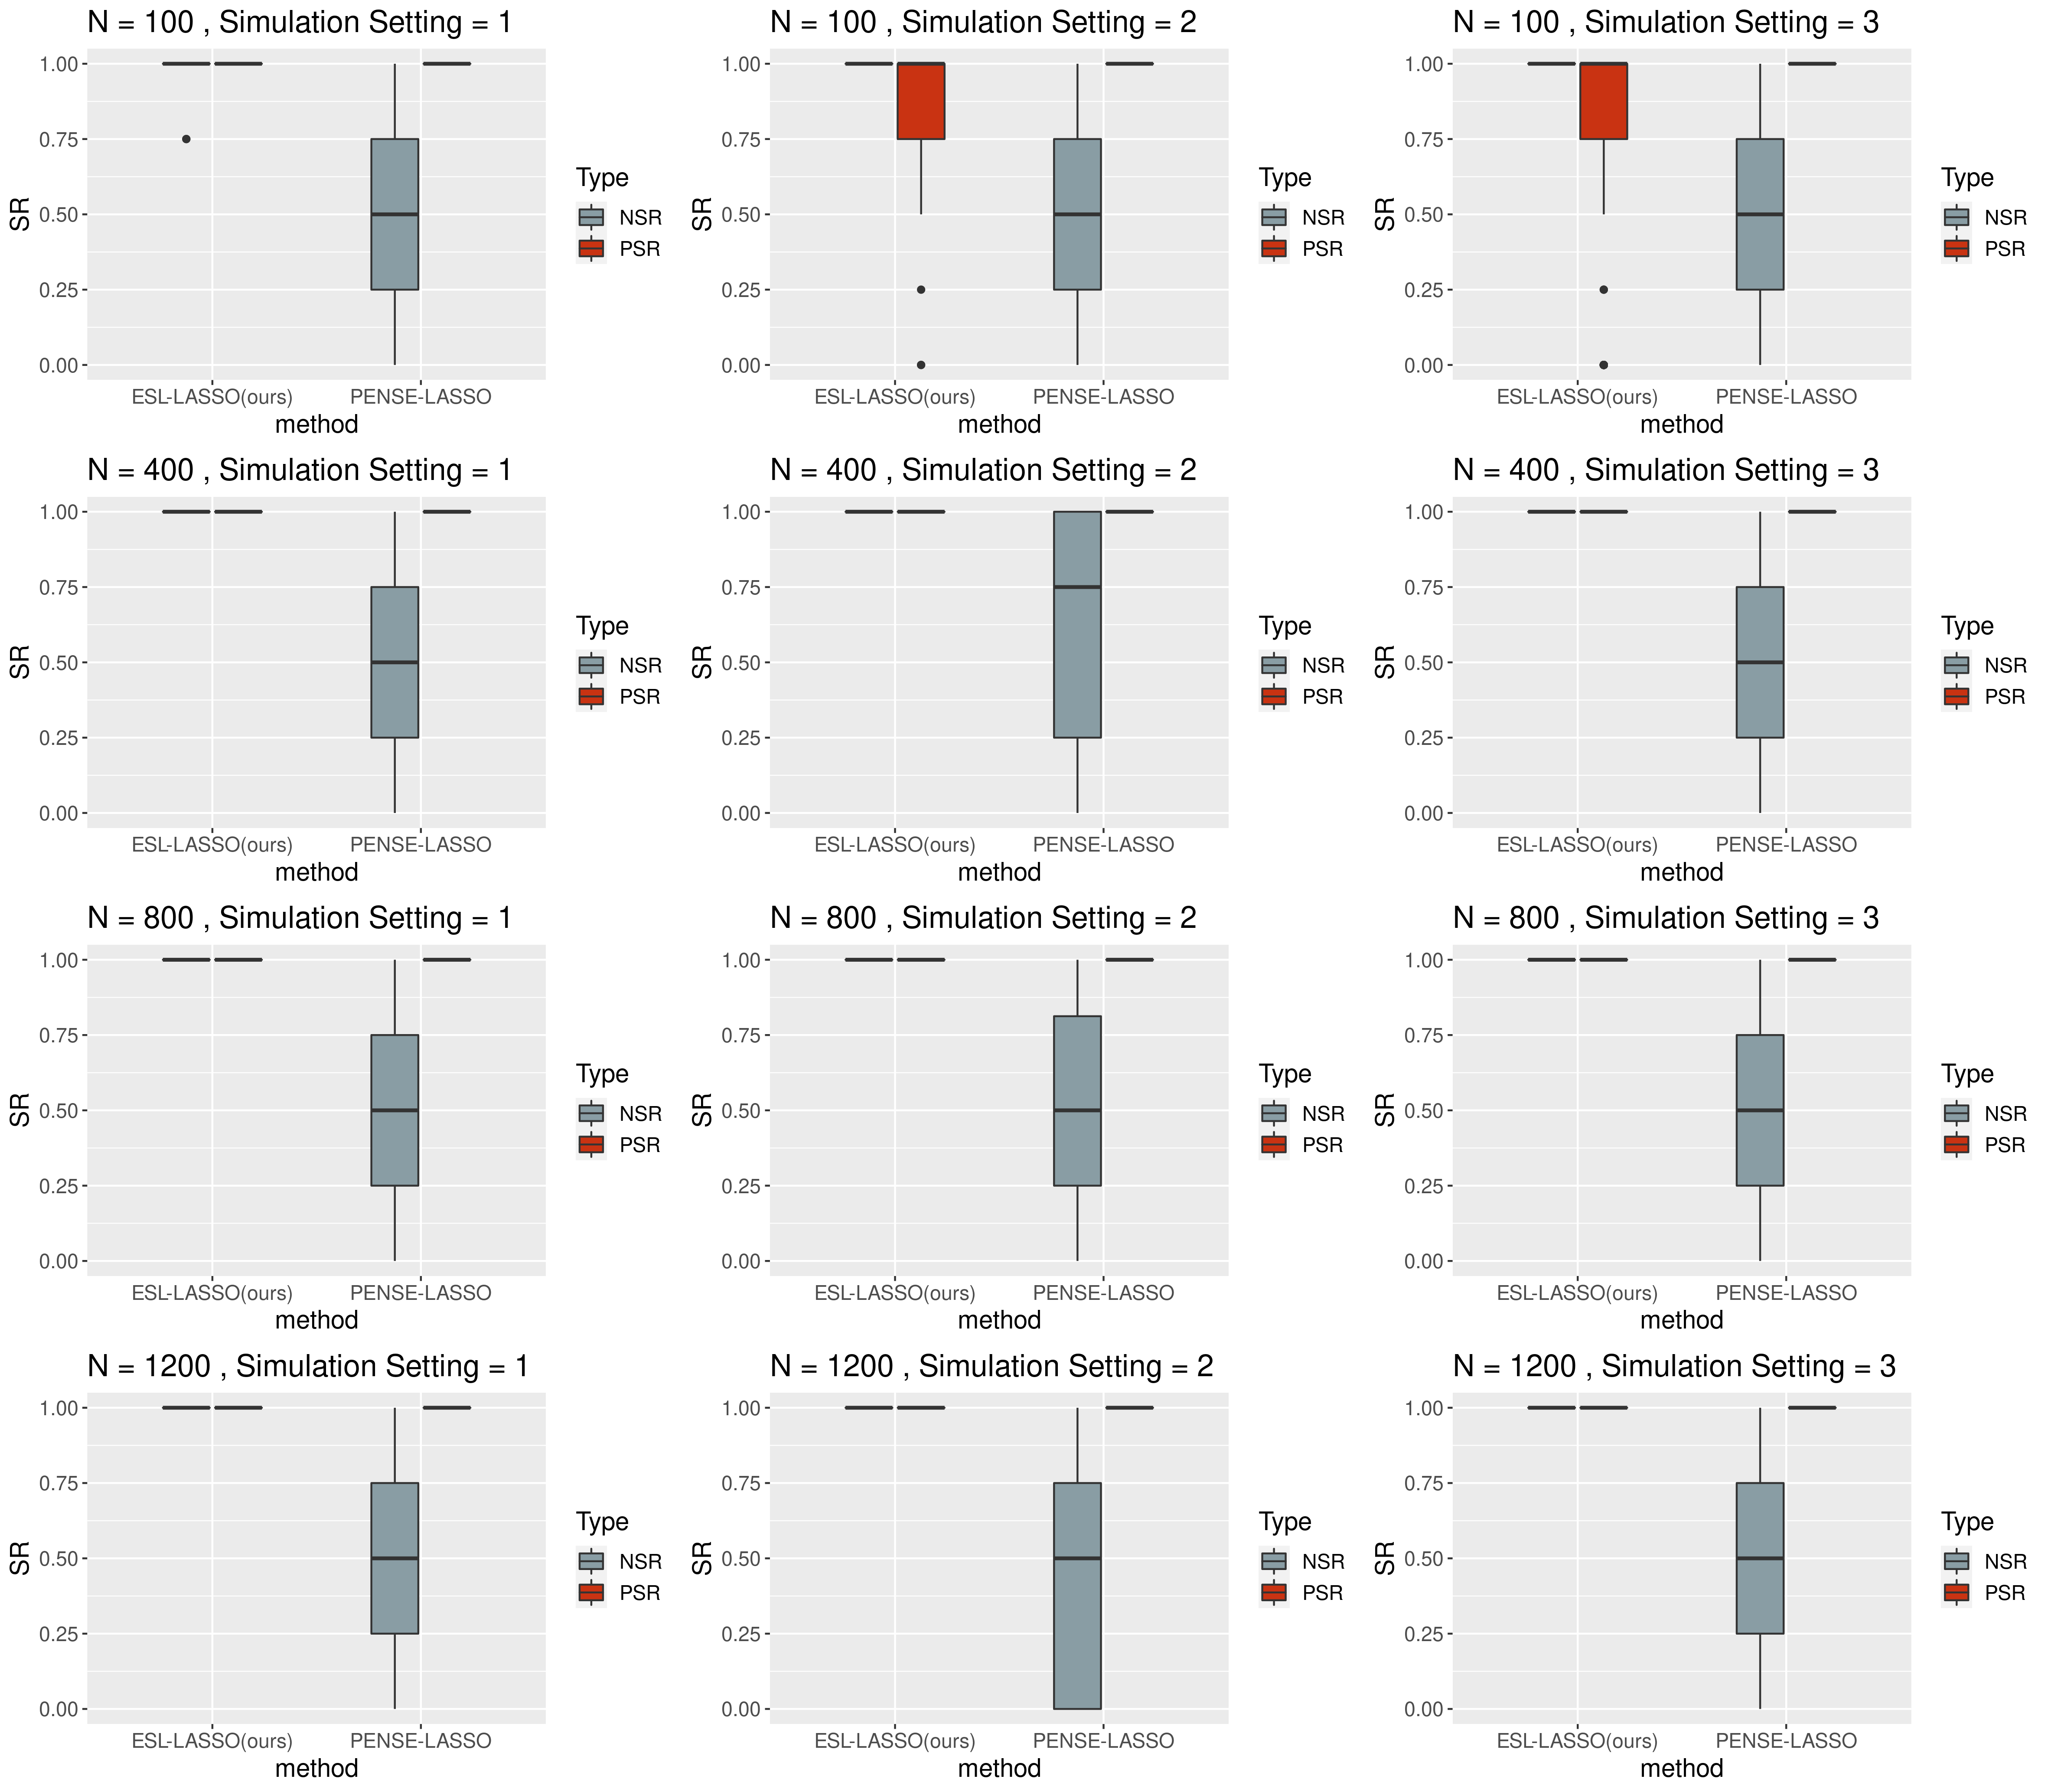
\includegraphics[width = \linewidth]{figures/SR_compare.png}
    \caption{Box plots for the variable selection rate across all simulation settings. }
    \label{fig:sr}
\end{figure}



\begin{figure}[t]
    \centering
    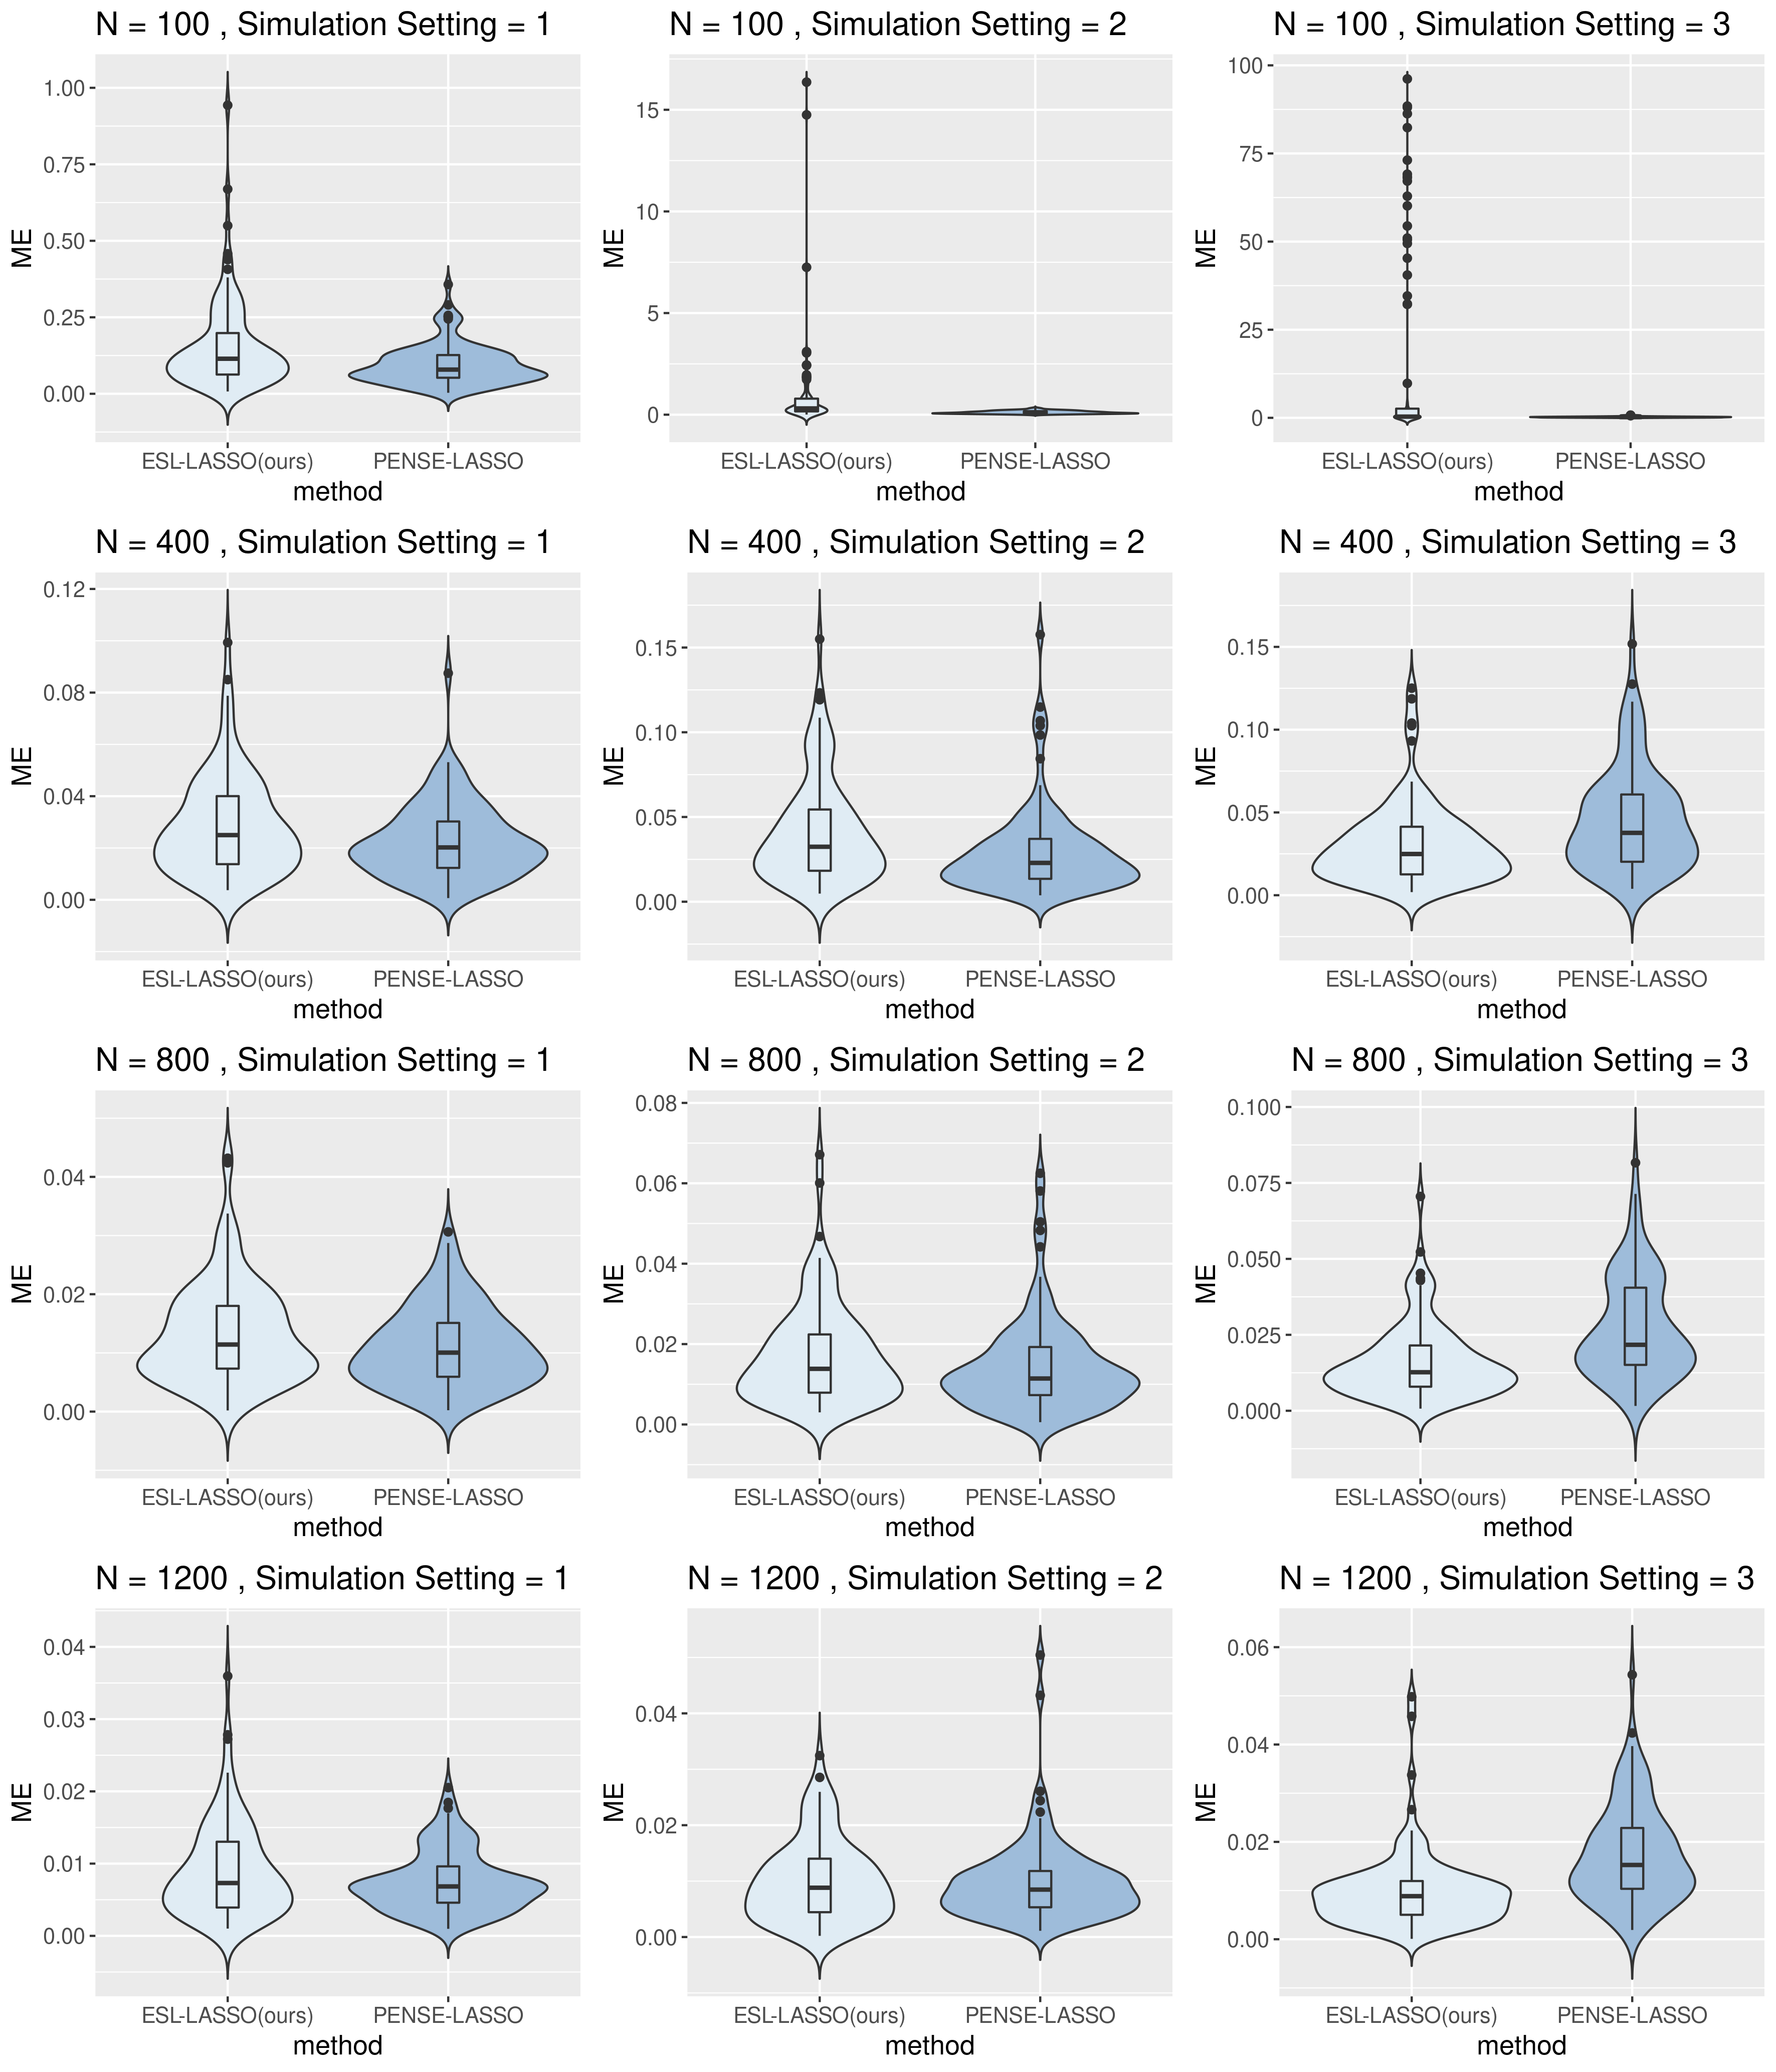
\includegraphics[width = \linewidth]{figures/ME_compare.png}
    \caption{Violin plots for the ME across all simulation settings. For each subfigure, the violin plot places two kernel density vertically with a box plot in the center. }
    \label{fig:me}
\end{figure}


In this section, we compare the quality of our version of ESL-LASSO (\cref{alg:esl_lasso}) with the LASSO version of PENSE \citep{freue2019robust} on three simulation settings that described in the paper. For each setting, we repeat both estimation methods for $100$ trials by generating $100$ datasets. And we test the performance of both methods across different samples sizes, i.e.,  $n = 100, 400, 800, 1200$.  
In general we set $d = 8$ and the true coefficients $\beta = \beta  =(1, 1.5, 2, 1, 0,0,0,0)^T$. 
We consider the following three data generating mechanisms:
\benum
\item Influential points in covariates: for $i = 1, 2, \dots, n$, 
\[
x_i &\distiid 0.8 \distNorm(0, I) + 0.2 \distNorm(3 \ind, \Omega), \quad [\Omega]_{i,j} = 0.5^{|i-j|}\\
\eps_i &\distiid \distNorm(0,1).
\]

\item Influential points in response: for $i = 1, 2, \dots, n$, 
\[
x_i &\distiid \distNorm(0\ind, \Omega), \quad [\Omega]_{i,j} = 0.5^{|i-j|}\\
\eps_i &\distiid 0.8\distNorm(0,1) + 0.2 \distNorm(10, 6^2).
\]

\item Influential points in both covariates and the response: for $i = 1, 2, \dots, n$, 
\[
x_i &\distiid 0.8 \distNorm(0, I) + 0.2 \distNorm(3 \ind, \Omega), \quad [\Omega]_{i,j} = 0.5^{|i-j|}\\
\eps_i &\distiid \distNamed{Cauchy}(0,1)
\]
\eenum


For ESL-LASSO, we repeat the complete procedure twice and base the proximal gradient descent with $50000$ iterations. For PENSE-LASSO, we use four-fold cross-validation to select the penalty constant that leads to the minimal mean square prediction error. In terms of the measure of performance, we evaluate both the variable selection precision---including PSR \citep{chen2008extended} and NSR \citep{fan2001variable}, which measures the proportion of true features selected by the methods and the proportion of discarded features with true zero coefficients respectively---and the model error proposed by the author, i.e.,
\[
\text{ME} = (\hat \beta - \beta_0)^T \left( \frac{1}{n} \sum_{i =1}^n x_i x_i^T\right)   (\hat \beta - \beta_0).
\]

As shown in \cref{fig:sr}, as sample size gets larger, ESL-LASSO shows better variable selection precision comparing to PENSE-LASSO, where both PSR and NSR are $1$ for $n =400, 800, 1200$. PENSE-LASSO is able to recover the true variables but have problem with discarding the variables with true zero coefficients. ESL-LASSO may benefit from the adaptive LASSO penalty while PENSE-LASSO uses the LASSO penalty, of which the performance may potentially be improved if we employ the same adaptive LASSO penalty to PENSE.
One may also notice that the performance of ESL-LASSO is not ideal when $n = 100$, such phenomenon is more clearly displayed in \cref{fig:me}, indicating that ESL-LASSO may suffer from numerical instability with small data size. 


Next, \cref{fig:me} gives a quantitative characterization of the relative performance of ESL-LASSO and PENSE-LASSO. As demonstrated in the plot,  in the first two simulation settings, ESL-LASSO displays a similar performance asymptotically as PENSE-LASSO. But in the third setting, where the influential points are introduced in both the covariates and the response,  ESL-LASSO behaves quite bad when $n  =100$ and gets slightly better than PENSE-LASSO as the sample size increases. 











